\section{Double counting}
\label{sec:doublecounting}

As it has been mentioned in the introduction, the ability to consistently include electro-weak correction in
PDF fits is not enough to make a fully-fledged fit possible in a consistent manner. Indeed, experimental data should
be provided in  a format that allows PDF collaborations to employ them in such fits in a theoretically sound manner. In this
section, we will try to provide some guidelines, by highlighting some sources of inconsistency commonly occurring in experimental 
analyses. These will either lead to accounting multiple times for EW effects (so-called double counting), or to not accounting at
all for such effects.\footnote{By no means we intend to blame on our beloved experimental colleagues for what they write or do. However,
    we think that by highlighting errors and making everybody more cautious about them is the only way to avoid repeating such
    errors in the future.}

A common source of inconsistency is the subtraction of (irreducible) background processes which must not be considered as such. The typical example
is neutral-current Drell--Yan, where the signal process is an opposite-sign lepton pair, which starts
at $\mathcal O(\alpha^2)$. Because this process is usually thought
as a quark-initiated, $s$-channel mechanism ($q\bar q \to \gamma^*/Z \to \ell^+ \ell^-$), in many analyses the photon-induced component,
$\gamma \gamma \to \ell^+ \ell^-$ in the $t$ channel, is considered as a different process, and it 
subtracted, possibly evaluated with different parton densities and/or including (unphysical) higher-order 
corrections. For example, in Refs.~\cite{Aaboud:2017ffb,Aad:2016zzw}, one reads:
\begin{quote}
The photon-induced process, $\gamma\gamma \to \ell \ell$, is simulated at LO using Pythia 8 
and the MRST2004qed PDF set~\cite{Martin:2004dh}. The expected yield for this process also accounts for 
NLO QED/EW corrections from references~\cite{Bardin:2012jk,Bondarenko:2013nu}, which decrease the yield by approximately 30\%.
\end{quote}
A similar statement appears also in an older analysis~\cite{Aad:2013iua}. Such a distinction cannot be physically
justified beyond LO\@. Indeed, at $\mathcal O(\alpha^3)$, the reaction $q \gamma \to \ell^+ \ell^- q$ becomes possible, which
includes both kind of topologies, see Fig.~\ref{fig:dy-pi}. 
\begin{figure}[ht!]
    \centering
    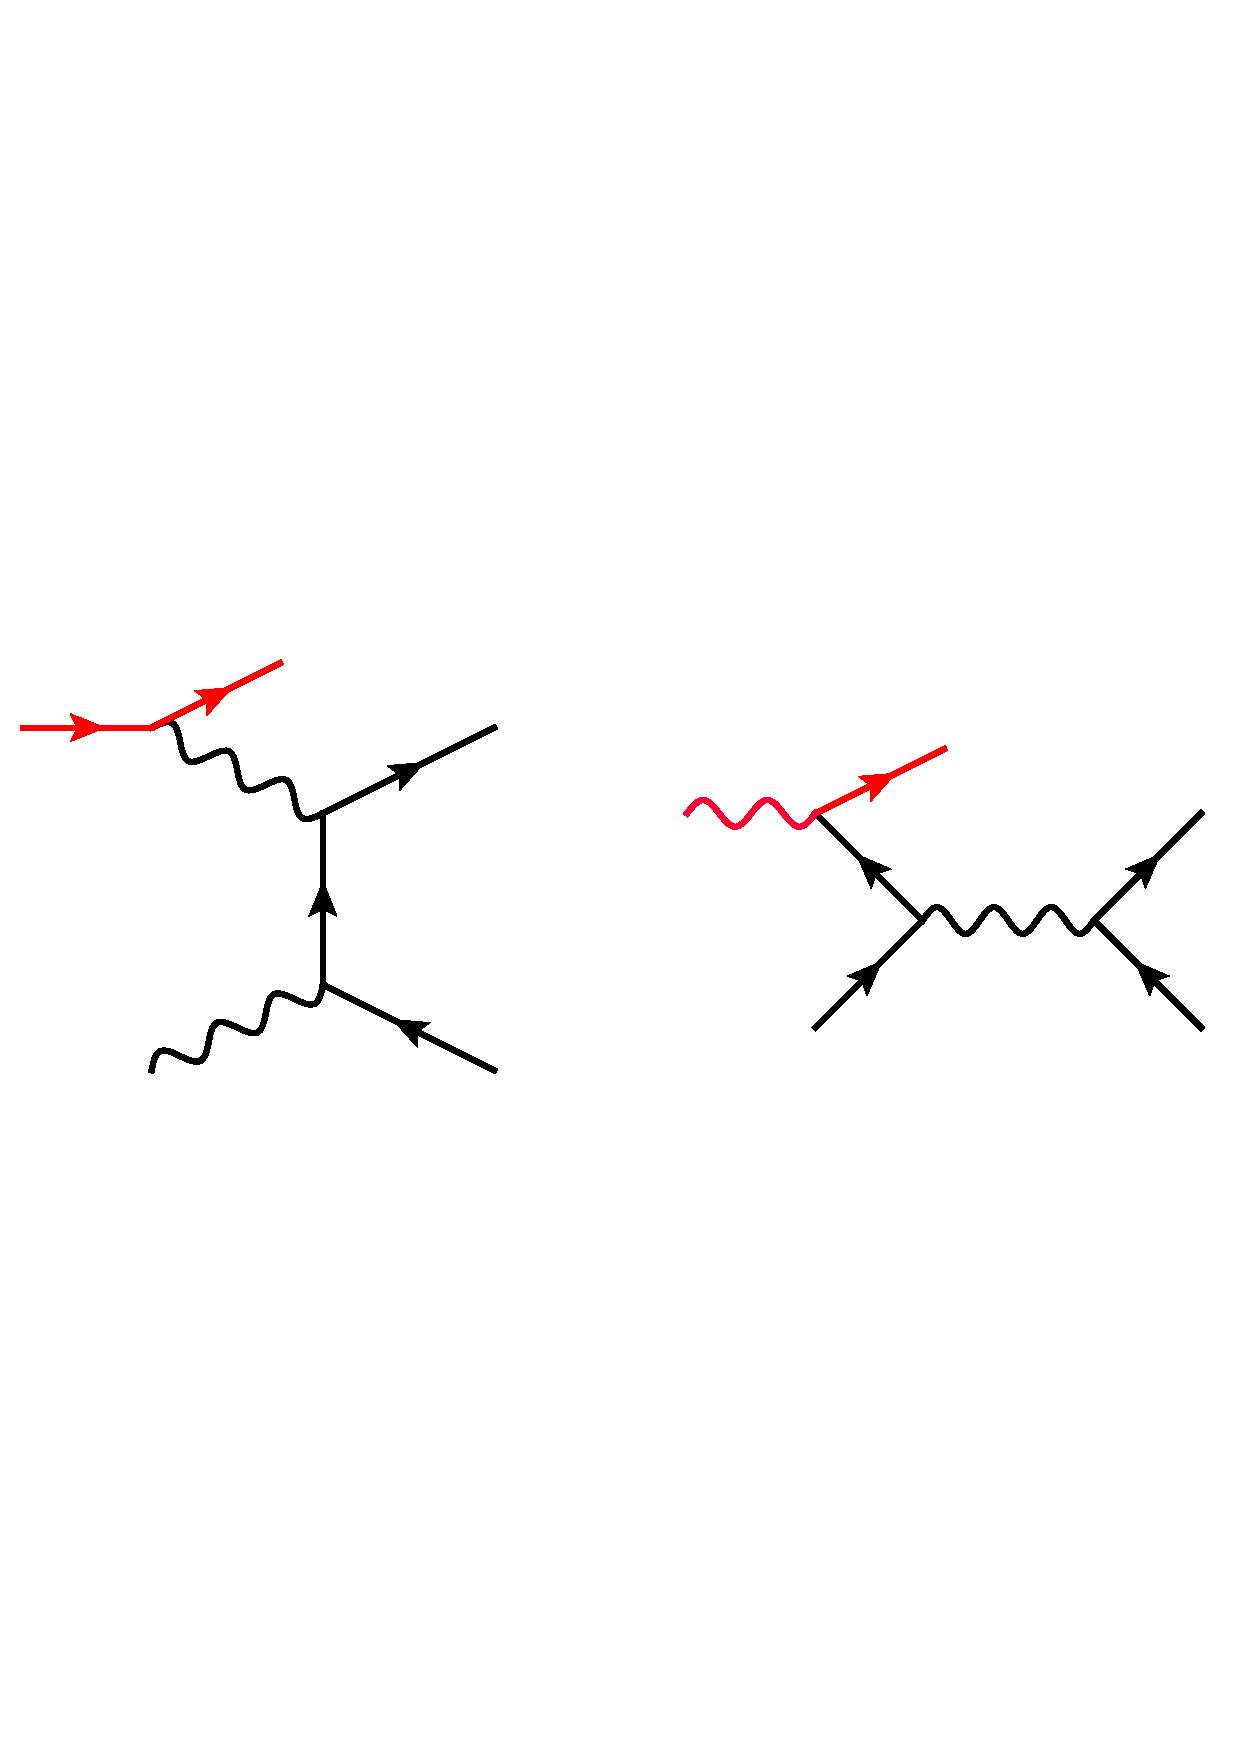
\includegraphics[width=0.6\textwidth, trim=0.cm 11cm 0.cm 2cm, clip=True]{figures/dy-pi.pdf}\\
    \caption{\label{fig:dy-pi}
    Photon-induced (left) and quark-induced (right) contributions to the Drell-Yan process. In black, the LO process is shown.
    In red, the initial-state splitting leading to the real-emission $q \gamma \to \ell^+ \ell^- q$ is highlighted. Such a 
    real emission enters in the NLO EW corrections.}
\end{figure}

{\bf It looks like CMS does things in a pretty consistent manner~\cite{Sirunyan:2018owv, CMS:2014jea}. Shall we mention? We should
not make ATLAS appear as the bad guys, and CMS as the good ones.} The problem here derives from the fact 
that identifying a process based only on its
initial-state partons is plain wrong in quantum mechanics. While this fact is well established in QCD---nobody would ever
consider to \enquote{subtract} the gluon-initiated contribution to top-pair production in top analyses---seemingly it is not so
when EW corrections are considered.

A second example is related to removing EW effects from data. These can be either the full EW corrections (Refs??) 
or just a part, for example deconvolving multiple-photon radiation from light particles in the final state. This applies mostly
to processes such as neutral- or charge-current Drell--Yan, specially when electrons are considered. The problem lie in the fact that
 electrons, and to a lesser extent muons, tend to radiate photons, and such photons are typically not accounted
for in hard matrix-elements. Thus, leptons that are measured in the detector are less energetic, and this fact is compensated for
by undoing the photon shower before publishing data, which are referred to e.g.\ as \emph{Born-level electrons}~\cite{}. There are
at least two 
problems related with this. The first, a quite obvious one, is that when EW corrections
are included at fixed order, the first photon emission is included exactly at the matrix-element level. The second, which
applies for electrons, is that they are never measured as bare particles, because of the finite resolution 
of the electromagnetic calorimeter. Since collinear photonic emission cannot be resolved, at least data 
involving electrons should also be published
in terms of dressed particles, after applying some recombination scheme. This has the further advantage of being 
inclusive on the effect of further collinear emissions. For what concerns muons, while in principle
the concept of bare muons is a physical one, it should be kept in mind that modern, general-purpose codes employed to
compute EW corrections treat leptons as massless. This fact encourages to explore the possibility of employing dressed
muons, on the same footing as their electron counterpart.

\clearpage
\noindent
\textbf{Notes from CS}:
\begin{itemize}
\item overall we should also point out the positive (rewrite the last part of this section a bit): for leptonic observables there always seems to be a pre-/post-FSR dataset with born/dressed leptons
\begin{itemize}
\item is this really the case?
\item is this also the case for non-leptonic observables? Specifically: Do ATLAS/CMS subtract photon radiation for observables of jet, top, or any other reconstructed objects (for instance: Z pT)?
\end{itemize}
\item double-photon initiated processes:
\begin{itemize}
\item how do they subtract it exactly (one analysis uses a concrete PDF set and subtracts the theory prediction; point out first how they do it, then that this is not a good idea, even if it would make sense: mixing theory predictions with measurements)
\item explain why they do it and point that this is not good
\end{itemize}
\item stress subtraction of \emph{irreducible} backgrounds
\end{itemize}
